\documentclass[a4paper,UTF8]{article}
\usepackage{ctex}
\usepackage[margin=1.25in]{geometry}
\usepackage{color}
\usepackage{graphicx}
\usepackage{amssymb}
\usepackage{amsmath}
\usepackage{amsthm}
%\usepackage[thmmarks, amsmath, thref]{ntheorem}
\theoremstyle{definition}
\newtheorem*{solution}{Solution}
\newtheorem*{prove}{Proof}
\usepackage{multirow}
\usepackage{url}
\usepackage{enumerate}
\usepackage{algorithm}
\usepackage{algorithmic}
\usepackage{caption}
\usepackage{subcaption}
\usepackage{booktabs}
\usepackage{listings}
\renewcommand{\algorithmicrequire}{\textbf{Input:}}
\renewcommand{\algorithmicensure}{\textbf{Procedure:}}
\renewcommand\refname{参考文献}

%--

%--
\begin{document}
\title{实验3. 强化学习实践}
\author{MG1733098, 周华平, \url{zhp@smail.nju.edu.cn}}
\maketitle

\section*{综述}



\section*{实验二.}



\section*{实验三.}


\subsection*{Deep Q-network(DQN)实现}

在本实验中,我选择使用PyTorch来实现DQN。
在定义Q值网络时我使用了MLP,其中网络结构由3层Linear构成;激活函数使用PReLU,
同时在每个隐层中增加Batch Norm来对相应的activation做规范化操作。
另外,在DQN中我采用\lstinline[language=Python]{optim.Adam}作为优化函数,
用\lstinline[language=Python]{nn.MSELoss()}来计算均方误差。

Q值网络的定义如下所示:

\begin{lstlisting}[language=Python]
class DQN(nn.Module):
    def __init__(self, input_dim, output_dim, hidden_dim):
        super(DQN, self).__init__()
        self.layer1 = nn.Sequential(
            nn.Linear(input_dim, hidden_dim),
            nn.BatchNorm1d(hidden_dim),
            nn.PReLU(),
        )
        self.layer2 = nn.Sequential(
            nn.Linear(hidden_dim, hidden_dim),
            nn.BatchNorm1d(hidden_dim),
            nn.PReLU(),
        )
        self.out = nn.Linear(hidden_dim, output_dim)

    def forward(self, x):
        x = self.layer1(x)
        x = self.layer2(x)
        return self.out(x)
\end{lstlisting}

\subsection*{CartPole}

针对CartPole,DQN的超参数设置如表\ref{tab:pole-dqn}所示。
% TODO 公式ref
其中$\epsilon$的衰减公式同公式(abcd)。

\begin{table}[H]
	\centering
	\begin{tabular}{ccc}
		\toprule
		超参数 & 参数意义 & 参数值 \\
		\midrule
		memory\_size & Replay Memory的大小 & 10000 \\
		batch\_size & mini-batch的大小 & 128 \\
		hidden\_dim & DQN的隐层维度 & 50 \\
		discount & DQN算法中的$\gamma$ & 0.99 \\
		learning\_rate & DQN算法中的$\alpha$ & 0.001 \\
		eps\_start & $\epsilon$的初始值 & 0.9 \\
		eps\_end & $\epsilon$的结束值 & 0.05 \\
		eps\_decay & $\epsilon$的衰减权重 & 200 \\
		\bottomrule
	\end{tabular}
	\caption{DQN超参数设置(CartPole)}\label{tab:pole-dqn}
\end{table}

DQN在CartPole上的实验结果如图\ref{fig:pole-dqn}所示。
%TODO 说明图中的信息
可以观察到Loss在超过450轮后达到收敛的状态。
由于$\epsilon$的最小值被设置为0.05,因此即使Training了较多轮数,
DQN依旧会以5\%的概率随机选择Action。
而CartPole似乎对于错误的Action比较敏感,
当随机到错误的Action时,可能会导致该轨迹提前结束。
因此在Training阶段Reward似乎并没有收敛到一个固定值,
然而我们可以观察到随着Training轮数的增加,
Reward的上限也在不断提高,这也从侧面体现出了训练是有效果的。

\begin{figure}[H]
	\centering
	\begin{subfigure}[t]{0.5\textwidth}
		\centering
		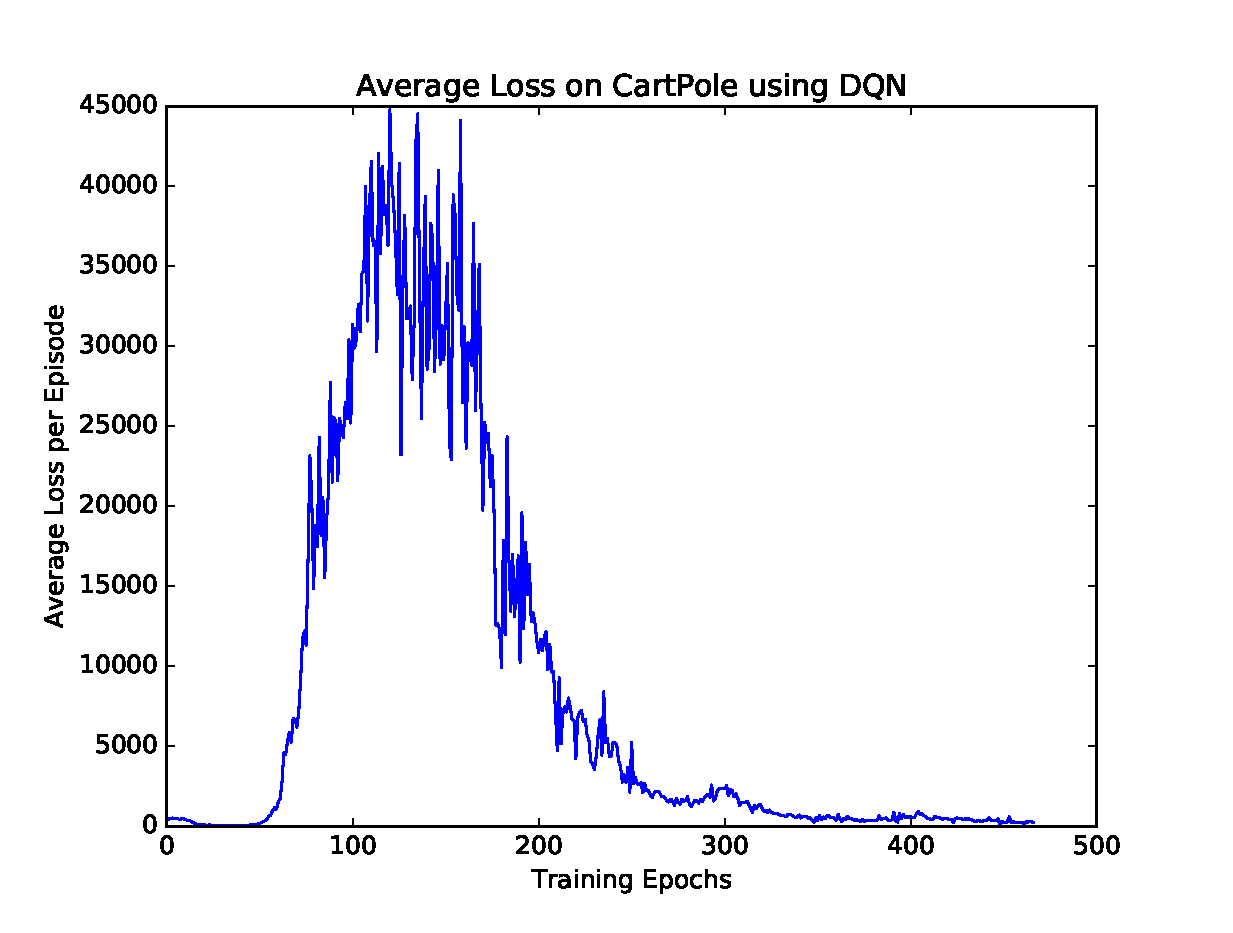
\includegraphics[scale=0.35]{figures/pole-dqn-loss}
		\caption{Average Loss}
	\end{subfigure}%
	\begin{subfigure}[t]{0.5\textwidth}
		\centering
		\includegraphics[scale=0.35]{figures/pole-dqn-reward}
		\caption{Average Reward}
	\end{subfigure}
	\caption{Training Result of CartPole using DQN}\label{fig:pole-dqn}
\end{figure}


\subsection*{MountainCar}

针对MountainCar,DQN的超参数设置如表\ref{tab:car-dqn}所示。

\begin{table}[H]
	\centering
	\begin{tabular}{ccc}
		\toprule
		超参数 & 参数意义 & 参数值 \\
		\midrule
		memory\_size & Replay Memory的大小 & 10000 \\
		batch\_size & mini-batch的大小 & 128 \\
		hidden\_dim & DQN的隐层维度 & 50 \\
		discount & DQN算法中的$\gamma$ & 0.99 \\
		learning\_rate & DQN算法中的$\alpha$ & 0.001 \\
		eps\_start & $\epsilon$的初始值 & 0.9 \\
		eps\_end & $\epsilon$的结束值 & 0.05 \\
		eps\_decay & $\epsilon$的衰减权重 & 50 \\
		\bottomrule
	\end{tabular}
	\caption{DQN超参数设置(MountainCar)}\label{tab:car-dqn}
\end{table}

DQN在MountainCar上的实验结果如图\ref{fig:car-dqn}所示。
其中Reward在超过200轮之后达到收敛的状态,
而Loss也在超过200轮之后达到了基本稳定的状态。

\begin{figure}[H]
	\centering
	\begin{subfigure}[t]{0.5\textwidth}
		\centering
		\includegraphics[scale=0.35]{figures/car-dqn-loss}
		\caption{Average Loss}
	\end{subfigure}%
	\begin{subfigure}[t]{0.5\textwidth}
		\centering
		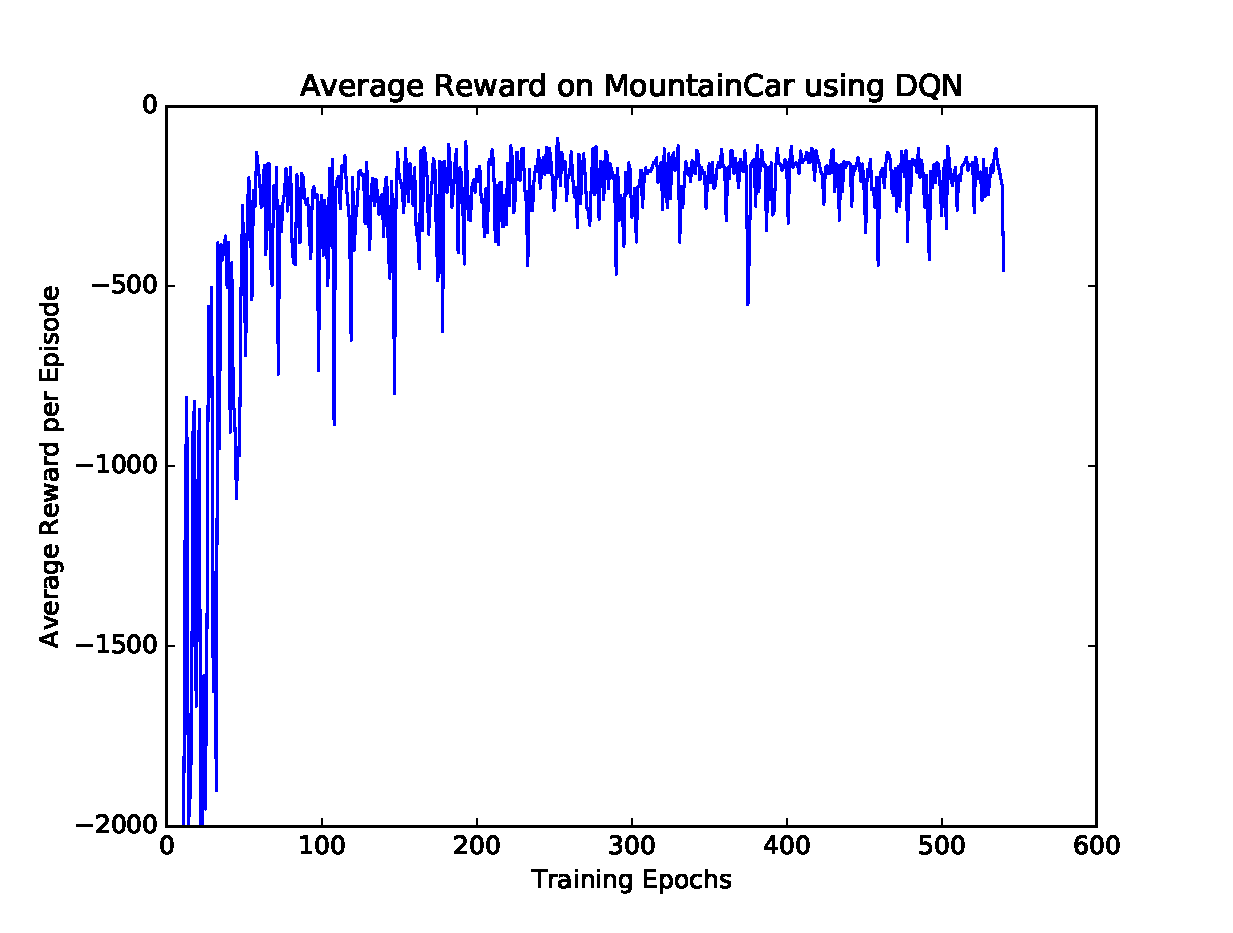
\includegraphics[scale=0.35]{figures/car-dqn-reward}
		\caption{Average Reward}
	\end{subfigure}
	\caption{Training Result of MountainCar using DQN}\label{fig:car-dqn}
\end{figure}

\subsection*{Acrobot}

针对Acrobot,DQN的超参数设置如表\ref{tab:bot-dqn}所示。

\begin{table}[H]
	\centering
	\begin{tabular}{ccc}
		\toprule
		超参数 & 参数意义 & 参数值 \\
		\midrule
		memory\_size & Replay Memory的大小 & 5000 \\
		batch\_size & mini-batch的大小 & 128 \\
		hidden\_dim & DQN的隐层维度 & 50 \\
		discount & DQN算法中的$\gamma$ & 0.99 \\
		learning\_rate & DQN算法中的$\alpha$ & 0.001 \\
		eps\_start & $\epsilon$的初始值 & 0.9 \\
		eps\_end & $\epsilon$的结束值 & 0.05 \\
		eps\_decay & $\epsilon$的衰减权重 & 200 \\
		\bottomrule
	\end{tabular}
	\caption{DQN超参数设置(Acrobot)}\label{tab:bot-dqn}
\end{table}

DQN在Acrobot上的实验结果如图\ref{fig:bot-dqn}所示。
在超过40轮之后,Loss达到了较低的水平,并且Reward也趋近于收敛。

\begin{figure}[H]
	\centering
	\begin{subfigure}[t]{0.5\textwidth}
		\centering
		\includegraphics[scale=0.35]{figures/bot-dqn-loss}
		\caption{Average Loss}
	\end{subfigure}%
	\begin{subfigure}[t]{0.5\textwidth}
		\centering
		\includegraphics[scale=0.35]{figures/bot-dqn-reward}
		\caption{Average Reward}
	\end{subfigure}
	\caption{Training Result of Acrobot using DQN}\label{fig:bot-dqn}
\end{figure}

\section*{实验四.}

\subsection*{CartPole}

针对CartPole,Improved DQN的超参数设置如表\ref{tab:pole-idqn}所示。

\begin{table}[H]
	\centering
	\begin{tabular}{ccc}
		\toprule
		超参数 & 参数意义 & 参数值 \\
		\midrule
		memory\_size & Replay Memory的大小 & 5000 \\
		batch\_size & mini-batch的大小 & 128 \\
		hidden\_dim & DQN的隐层维度 & 50 \\
		target\_c & $\hat{Q}$的更新频率 & 10 \\
		discount & DQN算法中的$\gamma$ & 0.99 \\
		learning\_rate & DQN算法中的$\alpha$ & 0.001 \\
		eps\_start & $\epsilon$的初始值 & 0.9 \\
		eps\_end & $\epsilon$的结束值 & 0.05 \\
		eps\_decay & $\epsilon$的衰减权重 & 200 \\
		\bottomrule
	\end{tabular}
	\caption{Improved DQN超参数设置(CartPole)}\label{tab:pole-idqn}
\end{table}

Improved DQN在CartPole上的实验结果如图\ref{fig:pole-idqn}所示。
% TODO 介绍结果以及和DQN的区别

\begin{figure}[htbp]
	\centering
	\begin{subfigure}[t]{0.5\textwidth}
		\centering
		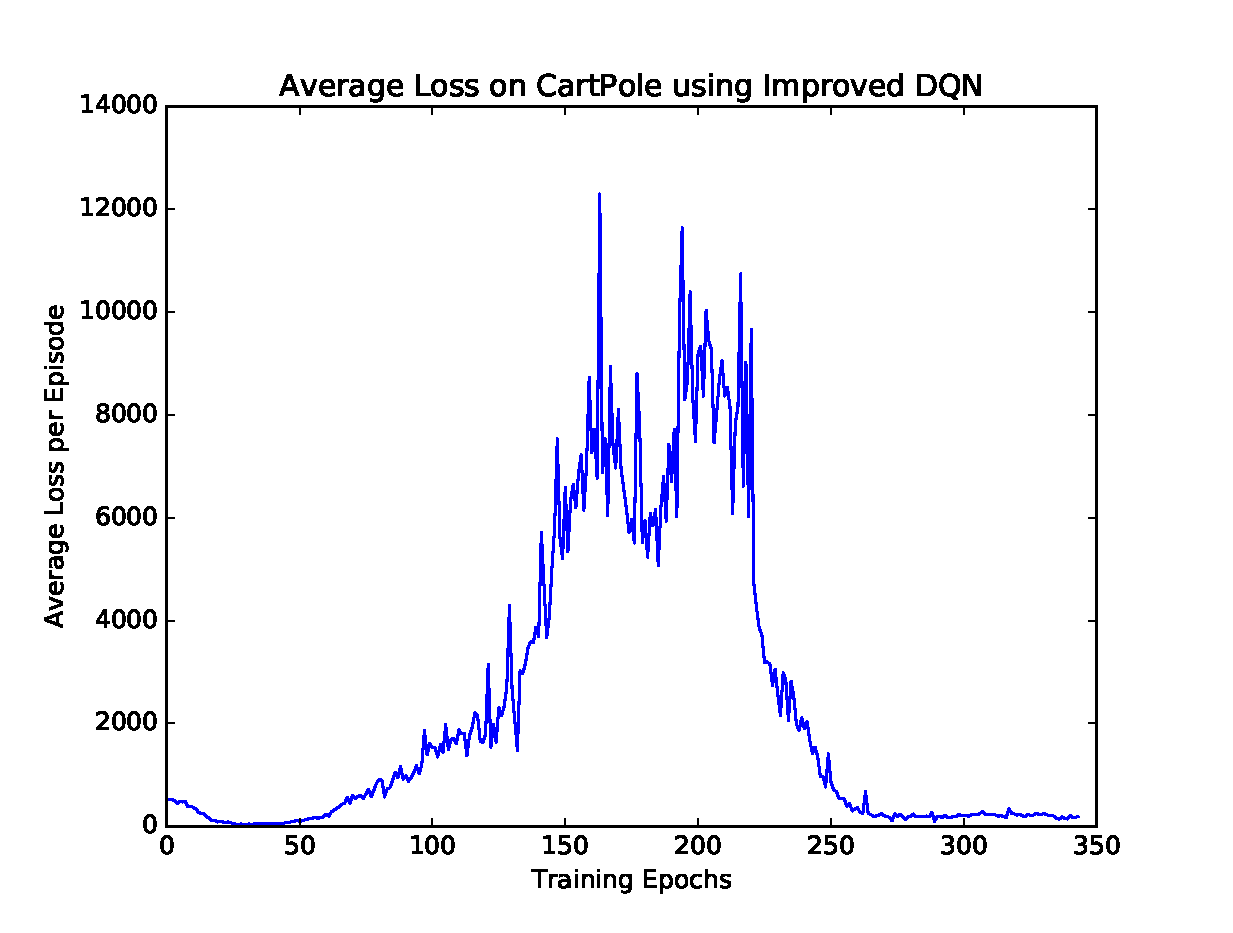
\includegraphics[scale=0.35]{figures/pole-idqn-loss}
		\caption{Average Loss}
	\end{subfigure}%
	\begin{subfigure}[t]{0.5\textwidth}
		\centering
		\includegraphics[scale=0.35]{figures/pole-idqn-reward}
		\caption{Average Reward}
	\end{subfigure}
	\caption{Training Result of CartPole using Improved DQN}\label{fig:pole-idqn}
\end{figure}


\subsection*{MountainCar}

\begin{table}[H]
	\centering
	\begin{tabular}{ccc}
		\toprule
		超参数 & 参数意义 & 参数值 \\
		\midrule
		memory\_size & Replay Memory的大小 & 5000 \\
		batch\_size & mini-batch的大小 & 128 \\
		hidden\_dim & DQN的隐层维度 & 50 \\
		target\_c & $\hat{Q}$的更新频率 & 10 \\
		discount & DQN算法中的$\gamma$ & 0.99 \\
		learning\_rate & DQN算法中的$\alpha$ & 0.001 \\
		eps\_start & $\epsilon$的初始值 & 0.9 \\
		eps\_end & $\epsilon$的结束值 & 0.05 \\
		eps\_decay & $\epsilon$的衰减权重 & 50 \\
		\bottomrule
	\end{tabular}
	\caption{Improved DQN超参数设置(MountainCar)}\label{tab:car-idqn}
\end{table}

Improved DQN在MountainCar上的实验结果如图\ref{fig:car-idqn}所示。

\begin{figure}[htbp]
	\centering
	\begin{subfigure}[t]{0.5\textwidth}
		\centering
		\includegraphics[scale=0.35]{figures/car-idqn-loss}
		\caption{Average Loss}
	\end{subfigure}%
	\begin{subfigure}[t]{0.5\textwidth}
		\centering
		\includegraphics[scale=0.35]{figures/car-idqn-reward}
		\caption{Average Reward}
	\end{subfigure}
	\caption{Training Result of MountainCar using Improved DQN}\label{fig:car-idqn}
\end{figure}

\subsection*{Acrobot}

\begin{table}[H]
	\centering
	\begin{tabular}{ccc}
		\toprule
		超参数 & 参数意义 & 参数值 \\
		\midrule
		memory\_size & Replay Memory的大小 & 10000 \\
		batch\_size & mini-batch的大小 & 128 \\
		hidden\_dim & DQN的隐层维度 & 50 \\
		target\_c & $\hat{Q}$的更新频率 & 5 \\
		discount & DQN算法中的$\gamma$ & 0.99 \\
		learning\_rate & DQN算法中的$\alpha$ & 0.001 \\
		eps\_start & $\epsilon$的初始值 & 0.9 \\
		eps\_end & $\epsilon$的结束值 & 0.05 \\
		eps\_decay & $\epsilon$的衰减权重 & 200 \\
		\bottomrule
	\end{tabular}
	\caption{Improved DQN超参数设置(Acrobot)}\label{tab:bot-idqn}
\end{table}

Improved DQN在Acrobot上的实验结果如图\ref{fig:bot-idqn}所示。

\begin{figure}[htbp]
	\centering
	\begin{subfigure}[t]{0.5\textwidth}
		\centering
		\includegraphics[scale=0.35]{figures/bot-idqn-loss}
		\caption{Average Loss}
	\end{subfigure}%
	\begin{subfigure}[t]{0.5\textwidth}
		\centering
		\includegraphics[scale=0.35]{figures/bot-idqn-reward}
		\caption{Average Reward}
	\end{subfigure}
	\caption{Training Result of Acrobot using Improved DQN}\label{fig:bot-idqn}
\end{figure}

\end{document}
